\apendice{Plan de proyecto software}

\section{Introducción}

Existen dos temas a tratar en este apéndice. 
El primero corresponde a la planificación temporal del trabajo, en la cual veremos las tareas realizadas y los tiempos requeridos para llevarlas a cabo. También veremos el tiempo total necesario para la realización de este proyecto.  \\
El segundo tema que se va a desarrollar, es la realización de un análisis de la viabilidad de un proyecto de estas características en la vida real. Para ello nos centraremos en analizar las variables económicas y legales referentes al desarrollo de este trabajo. En cuanto a este último punto veremos los tipos de licencias que se pueden utilizar en este tipo de software


\section{Planificación temporal}

Como ya hemos comentado, la planificación del proyecto se llevó a cabo siguiendo la metodología SCRUM que está basada entre otras cosas, en el uso de \extranjerismo{sprints} para organizar la carga de tareas. 

Según esta metodología, estos sprints deben durar entre 1 y 3 semanas. Puesto que se está utilizando una metodología SCRUM, algunos tiempos pueden no ajustarse lo suficiente a lo esperado sobre todo los de los primeros sprint realizados, ya que en estos se debe llevar un proceso de medición de fuerzas y dificultades del trabajo a realizar. En este caso y puesto que mi situación personal ha sido distinta a lo largo de este proceso, la duración de estos sprints no ha sido siempre la misma. Esto se debe a que mis obligaciones han ido variando a medida que avanzaba el cuatrimestre. Al principio de este, durante los 3 primeros Sprint y comienzos del cuarto, disponía de bastante más tiempo para su realización por lo que era capaz de dedicar más horas al día. Posteriormente empecé a cursar las prácticas curriculares con un total de seis horas diarias lo que dificultó seguir con el mismo ritmo de dedicación al TFG. Se ha tratado de que los sprints estuvieran formados por aproximadamente el mismo número de horas. Estas horas están expuestas en el repositorio de GitHub y cada tarea tiene asignado un \extranjerismo{tag}. Cada uno de estos \extranjerismo{tags} es un número que relaciona 1 a 1 la dificultad con las horas para su realización, es decir, una dificultad de ocho equivale a aproximadamente 8 horas de trabajo. Como es lógico, cuanta mayor es la dificultad más se rompe esta relación, puesto que al ser más complicado, siempre suele alargarse el tiempo de realización de la tarea. 
El proyecto se desarrolló en los siguientes Sprints:
\begin{itemize}
\item Sprint 1. Investigación y familiarización (Software, Hardware y Herramientas)
\item Sprint 2. Envío y recepción de paquetes TCP/IP
\item Sprint 3. Investigación y primeros pasos con periféricos (Comunicación Uart, I2C)
\item Sprint 4. Investigación sobre Wifi. Uso de potenciómetros para gestionar motores
\item Sprint 5. Periféricos (sensor de temperatura y pantalla) y uso real en una empresa
\item Sprint 6. Memoria, presentación y últimos retoques
\end{itemize}
En los siguientes apartados obtendremos más información sobre como fue el desarrollo de cada uno de estos Sprints.


\subsection{Sprint 1}
Este Sprint está compuesto por 10 tareas que en total suman 43 puntos. Duró aproximadamente dos semanas. El comienzo fue complicado por la gran cantidad de conceptos y el funcionamiento del hardware que debí investigar, además de la dificultad de familiarizarse con dos IDEs diferentes. Las acciones principales fueron:
\begin{itemize}
\item Elección, descarga y familiarización del entorno de desarrollo.
\item Completar las prácticas propuestas por los tutores.
\item Descarga de otros programas para documentación, organización y comunicación.
\item Primeros pasos con lwIP.
\item Primeros pasos con RTOS.
\end{itemize}

%\imagen{Sprint1}{Tareas planificadas para el Sprint1.}
\begin{figure}[!h]
	\centering
	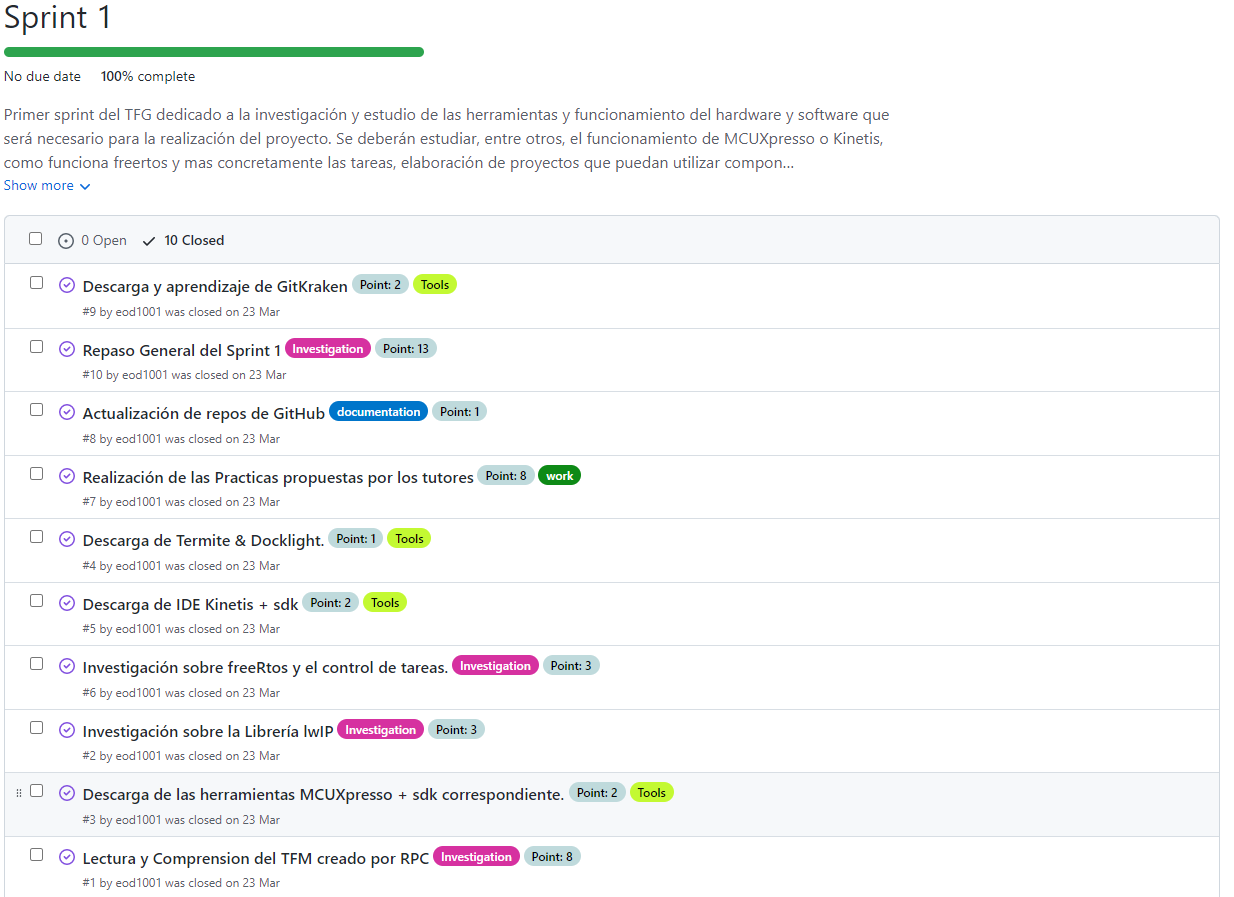
\includegraphics[width=0.9\textwidth]{Sprint1}
	\caption{Tareas planificadas para el Sprint1.}\label{sp1}
\end{figure}

Como podemos ver en la figura anterior, este primer Sprint se basó en la creación del entorno de trabajo y primeros pasos con las herramientas que iba a usar. Estos primeros pasos incluían ya la utilización de botones, leds y configuración de algún periférico.

\subsection{Sprint 2}
El sprint 2 recoge 9 tareas que suman 35 puntos de dificultad. Tuvo una duración de dos semanas y media. Este sprint estuvo enfocado a comenzar con la investigación del funcionamiento de lwIP. Cómo funcionaba y para qué servía, fueron los dos puntos más importantes. Tras entender estos dos puntos, busqué información sobre cómo implementarlo y comencé por la obtención de una IP según la mac de la placa y la creación de una tarea que pudiera recibir paquetes con información a través de este servicio. Para enviar los primeros paquetes utilicé Packet Sender.
\begin{itemize}
\item Investigación Protocolo TCP/IP y su implementación con lwIP.
\item Primeras partes del software.
\item Pruebas con la herramienta Packet Sender.
\end{itemize}

\imagen{Sprint2}{Tareas planificadas para el Sprint2.}


Otra parte a destacar fue el comienzo de la memoria con la herramienta Látex. Una herramienta que puede ser compleja de utilizar puesto que se debe aprender su sintaxis y acostumbrarse a un nuevo entorno para su uso.

\subsection{Sprint 3}
En este Sprint se buscó conseguir la comunicación de tres placas mediante el protocolo TCP/IP. En este punto, ya se disponía de conexión en red y de un \extranjerismo{`Listener'} que recibía paquetes de datos. El objetivo ahora era crear además, un \extranjerismo{`Writer'} capaz de enviarlos. Además, también se decidió la manera en que se transmitiría la información y sería en forma de comandos, por lo tanto también se implementó una especie de filtro que gestionaba el tipo de comando recibido en caso de existir. Por otro lado, también se comenzó a investigar e implementar las comunicaciones con los periféricos, concretamente con los motores y la pantalla. En este caso el sprint está constituido por 8 tareas que suman 36 puntos. Tareas principales:
\begin{itemize}
\item Creación del \extranjerismo{`Writer'}.
\item Creación del filtro de comandos.
\item Primeros pasos con UART y comunicación con los motores.
\item Primeros pasos con I2C y la pantalla LCD.
\end{itemize}

\imagen{Sprint3}{Tareas planificadas para el Sprint3.}

Este sprint tuvo una duración de dos semanas.

\subsection{Sprint 4}
En este Sprint se terminan, la comunicación de los motores y la de la pantalla, quedando operativas a falta de algunas mejoras. Además se produce uno de los hitos más importantes del proyecto, que es la investigación y abandono del procedimiento para la instalación del módulo wifi por falta de tiempo. En ese momento estaba comenzando las prácticas y se decide dejar apartada la parte de conexión inalámbrica para centrarme en la obtención de más funcionalidades. Esto viene dado porque desde la empresa en la que cursé las prácticas me ofrecieron la posibilidad de hacer algo que pudiera usarse en la fábrica.
Debido a esto, también me pongo a investigar sobre la posibilidad de introducir potenciómetros y sensores de temperatura para poder medir la temperatura de su CPD. El sprint suma una dificultad de 42 puntos en 8 tareas y se realizó en una semana y media. Tareas principales:
\begin{itemize}
\item Investigación sobre la implementación de un módulo WIFI, ESP8266.
\item Mejoras del código referente a la comunicación con los motores y la pantalla LCD.
\item Investigación e implementación de la lectura de los potenciómetros.
\end{itemize}

\imagen{Sprint4}{Tareas planificadas para el Sprint4.}

\subsection{Sprint 5}
Este sprint contiene 9 tareas llegando a un total de 32 puntos de dificultad. Es en este sprint donde se implementa la lectura del sensor de temperatura. Además se centran muchos esfuerzos en tratar de conseguir que todas las tareas funcionen adecuadamente. Se realizan multitud de pruebas y se trata de conseguir que la interacción con el usuario sea simple e intuitiva. Las tareas principales se resumen en:
\begin{itemize}
\item Mejora de usabilidad por el usuario.
\item Implementación del sensor de temperatura.
\item Mejora del código y funcionalidades de los periféricos.
\end{itemize}

\imagen{Sprint5}{Tareas planificadas para el Sprint5.}
La duración del sprint fue de una semana y media.
\subsection{Sprint 6}
Este Sprint se centra en dar los últimos retoques y completar la documentación a presentar para superar el TFG. Es el sprint más largo con 76 puntos de dificultad. En este caso se deberían haber separado en dos Sprints, pero puesto que todas las tareas se trataban sobre la documentación, se decidió dejar en solo uno. La duración de este sprint fue de dos semanas y media.
\begin{itemize}
\item Últimos retoques al código.
\item Generar la documentación de todo el trabajo.
\end{itemize}

\imagen{Sprint6}{Tareas planificadas para el Sprint6.}

\subsection{Diagrama de Gantt}
Para terminar con esta sección, se muestra el diagrama de Gantt seguido según la planificación temporal para la empresa, teniendo en cuenta festivos y fines de semana.

\begin{figure}[H]%
    \begin{center}%
    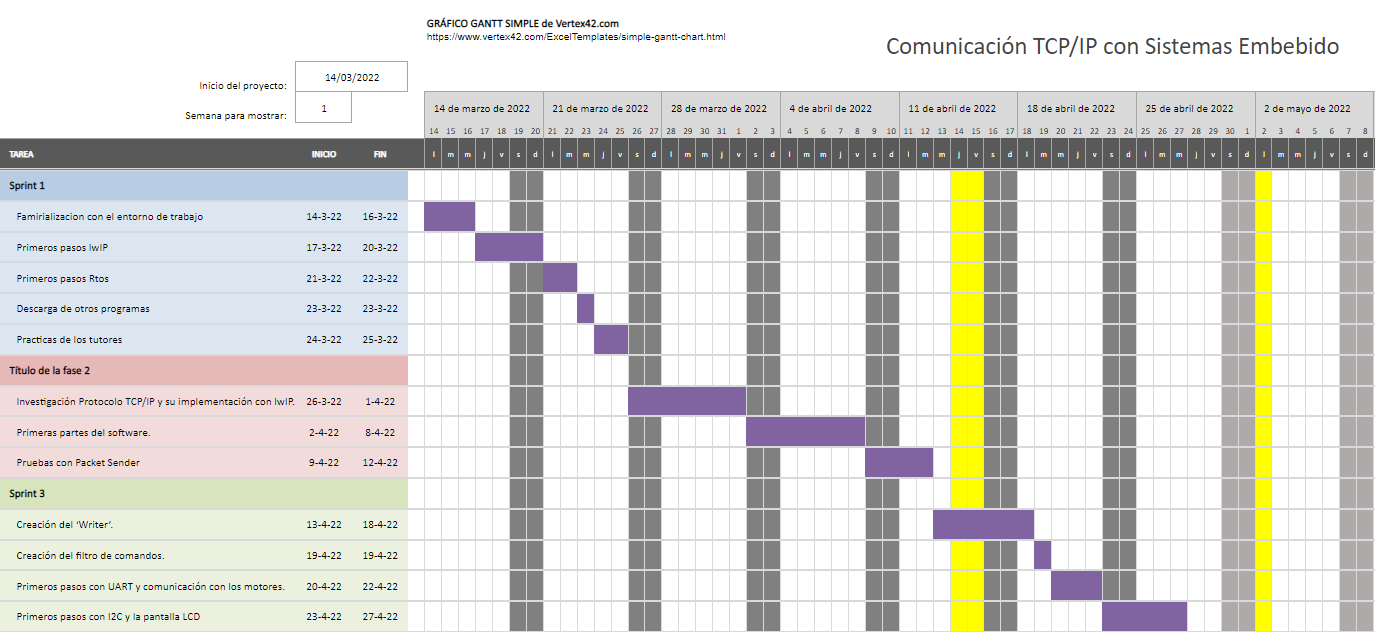
\includegraphics[angle=90,width=0.7\textwidth]{gantt1}%
    \caption{Diagrama de Gantt. Parte 1.}%
    \label{Dgantt1}%
    \end{center}%
  \end{figure}%
  
  \begin{figure}[H]%
    \begin{center}%
    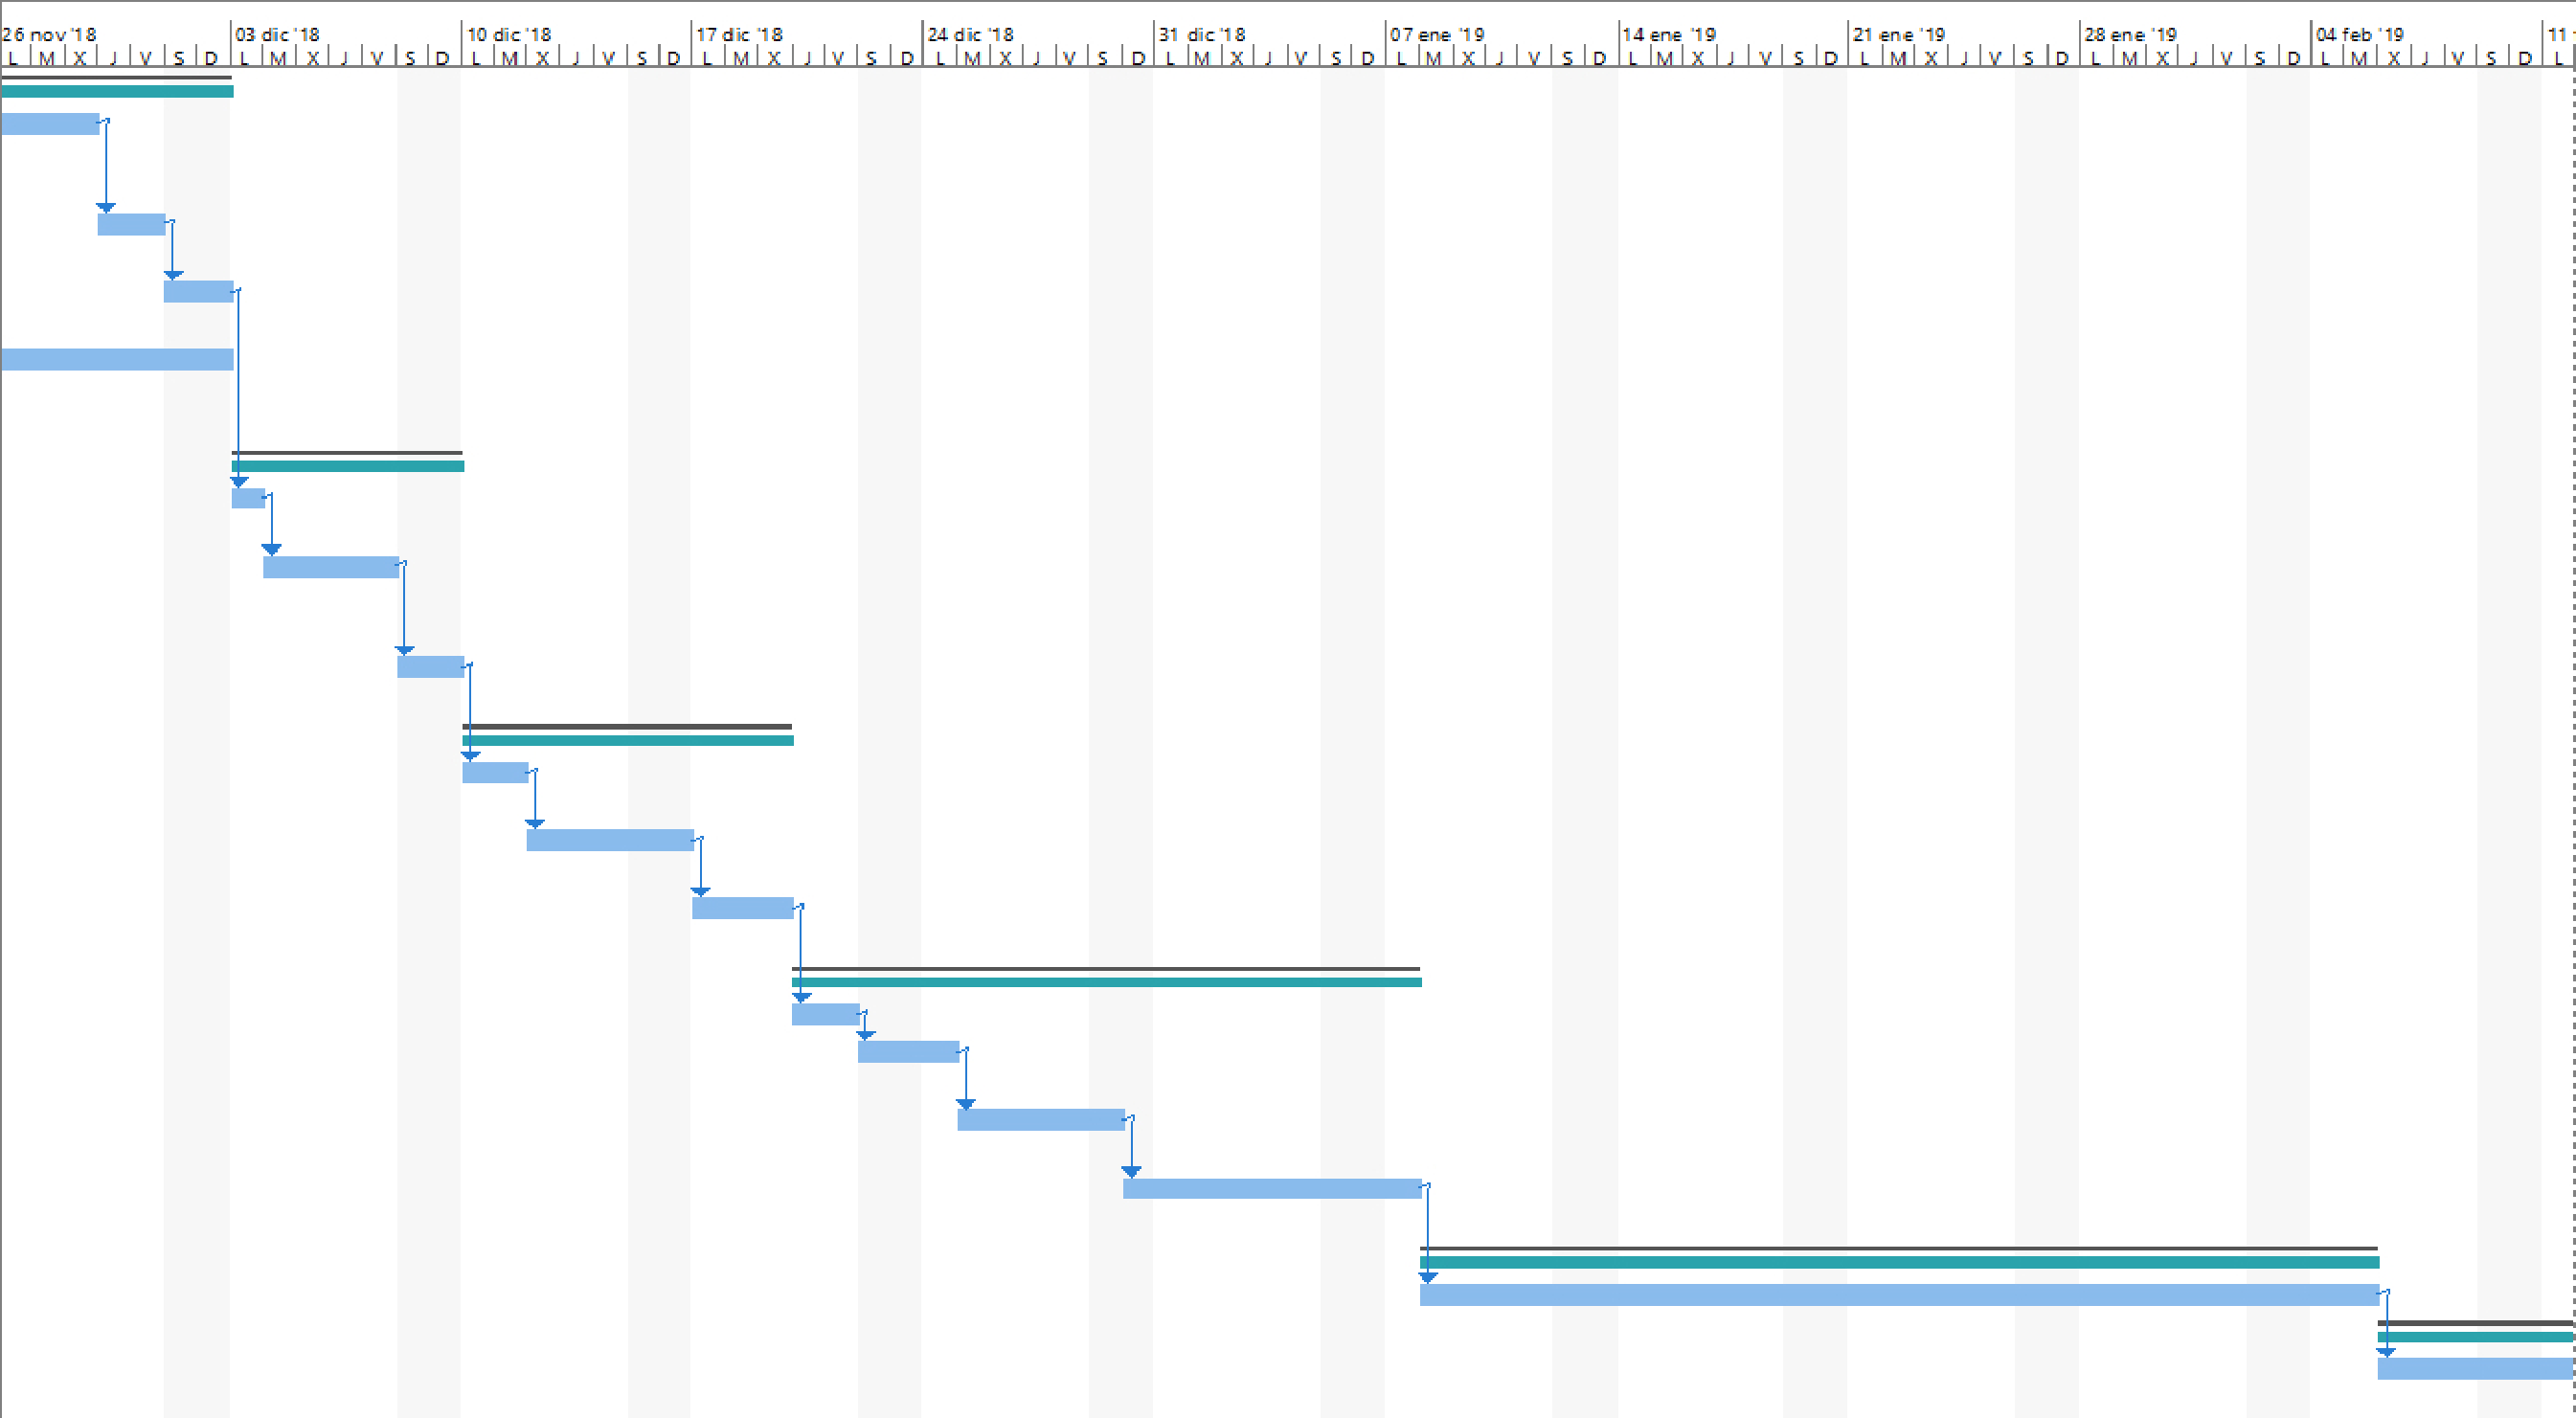
\includegraphics[angle=90,width=0.7\textwidth]{gantt2}%
    \caption{Diagrama de Gantt. Parte 2.}%
    \label{Dgantt2}%
    \end{center}%
  \end{figure}%

\section{Estudio de viabilidad}

\subsection{Viabilidad económica}
En este apartado se expone la viabilidad económica del desarrollo de este proyecto. Se tendrán en cuenta los gastos previstos durante el desarrollo y los beneficios, si los hubiera. Para calcularlo supondremos que el trabajo se hubiera desarrollado en el entorno real de una empresa. 

\subsubsection{Coste de personal.}
Para el desarrollo del producto final, vamos a suponer que se hubiera encargado una sola persona, durante un tiempo aproximado de 3 meses y 25 horas semanales. Supongamos que este trabajador junior tenga un salario bruto de 1500 euros al mes. 
Para conocer el salario neto lo haremos con la siguiente formula \cite{calculadoraSantander}:
\begin{equation} \label{eq:salario}
  salario\ bruto - IRPF - SS = salario\ neto
\end{equation}
Por lo que el trabajador recibiría el siguiente salario:
\begin{equation} \label{eq:salario}
  1500\text{\euro} - 10,49\% - 6,35\% = 1247,4\text{\euro}
\end{equation}
Para la realización de la fórmula anterior se han utilizado los tramos mas altos de la autonomía de Castilla y León \cite{escalaCyL} y la escala a nivel nacional que podemos encontrar en \cite{agenciaTributaria}. El cálculo está simplificado al no tener en cuenta la progresividad de la escala de tramos.


\subsubsection{Costes pertenecientes a la SS.}
Sobre el salario bruto, se producen retenciones y pagos a la Seguridad Social. De estos impuestos algunos los paga la empresa y otros el trabajador. En este apartado se van a calcular los importes de estas retenciones, para ello, tomaremos como referencia la tabla de bases de cotización de la Seguridad Social. En esta tabla, deberemos buscar el grupo que nos corresponda, en este caso ``Ingenieros y Licenciados. Personal de alta dirección no incluido en el artículo 1.3. c) del Estatuto de los Trabajadores''. Este grupo tiene unas bases mínimas de 1466,40€/mes. Y unas máximas de 4070,10€/mes.

\tablaSmallSinColores{Costes pertenecientes a la SS}{l l l}{costes-ss}
{\multicolumn{1}{l}{Concepto} & Empresa & Trabajador\\}
{
  Contingencias comunes & 23,60\% & 4,70\%\\
  Desempleo             &  5,50\% & 1,55\%\\
  FOGASA                &  0,20\% & 0,00\%\\
  Formación             &  0,60\% & 0,10\%\\
  \textbf{Total}        & \textbf{29,9\%} & \textbf{6,35\%}\\
}

Como podemos observar en la figura anterior los costes que la empresa debe asumir son el 29,9\% del salario del trabajador y el trabajador sufriría una retención del 6,35\% 

\subsubsection{Coste total de personal}
Para hallar el coste total del desarrollo del proyecto calcularemos la siguiente formula.
\begin{equation} \label{eq:salario}
  (salario\ mensual + costes\ ss) \times n^{o}\ meses = coste\ total
\end{equation}

De modo que el coste total se obtiene así:
\begin{equation} 
  (1500\text{\euro} + 448,5\text{\euro}) * 3 = 5845,5\text{\euro}
\end{equation}

La siguiente tabla recoge diferentes costes asociados al personal y 
su coste total.

\tablaSmallSinColores{Coste total de personal}{l l}{personal}
{\multicolumn{1}{l}{Concepto} & Coste\\}
{
  Salarios          & \EUR{1800}\\
  Seguridad Social  & \EUR{448,5}\\
  Meses             & 3 meses\\
  \textbf{Total}    & \textbf{\EUR{5845,5}}\\
}


\subsubsection{Costes del hardware.}
Como ya vimos en la memoria para el desarrollo de este proyecto, se han necesitado varios dispositivos. Aquí surge un inconveniente puesto que, según se recoge en la ley de impuestos sobre sociedades \cite{BasesyTiposSS} se necesitan 8 años para amortizar los equipos relacionados con la rama de la información, pero la renovación de este tipo de hardware se debe realizar en un periodo mucho menor, de 4 años. En este caso he optado por realizar los cálculos con un periodo de 4 años. Quedaría de la siguiente manera:

El coste mensual de un dispositivo se calcula así:
\begin{equation} \label{eq:coste-hw}
  Coste\ del\ dispositivo\ /\ Periodo\ de\ amortización\ (en\ meses)
\end{equation}

Por lo tanto, el coste de un dispositivo es el siguiente:
\begin{equation} \label{eq:coste-amor-hw}
  Coste\ mensual\ amortizado\ \times n^{o}\ meses\
\end{equation}

Para desarrollar cómodamente este software se ha utilizado una estación de trabajo portátil de 1000€ y un monitor de 24 pulgadas que tiene un coste de aproximadamente 150€.
\tablaSmallSinColores{Coste del \extranjerismo{hardware}}{l l l}{coste-hw}
{\multicolumn{1}{l}{\extranjerismo{Hardware}} & Coste & Coste amortizado\\}
{
  Entorno de trabajo & \EUR{1150} & \EUR{71,87}\\
  \textbf{Total}      & \EUR{1150} & \textbf{\EUR{71,87}}\\
}


\subsubsection{Costes del software.}

Para el desarrollo del proyecto, se han utilizado varios programas y aplicaciones. Según la ley del impuesto sobre sociedades \cite{ImpSoc}, el máximo de años para realizar la amortización de sistemas y programas informáticos es de 6 años. Sin embargo, al igual que hicimos en el apartado de los costes hardware, se calculará en un periodo de 4 años.
Es importante tener en cuenta que la mayoría de programas utilizados se encuentran bajo licencias que permiten su uso sin coste, por lo que no aparecerán en la tabla de costes de software.
Por otro lado, gran parte del software utilizado se usa mediante suscripción, por lo que su coste aparecerá computado bajo su suscripción determinada.

\tablaSmallSinColores{Coste del \extranjerismo{software}}{l l l}{coste-sw}
{\multicolumn{1}{l}
{\extranjerismo{Software}}              & Coste        & Coste amortizado\\}
{
  Windows 10 Pro\cite{win10pro} & \EUR{259}    & \EUR{21,58}\\
  Office 365\cite{office365}    & \EUR{126}    & \EUR{31,5}\\
  \textbf{Total}                        & \EUR{385} & \textbf{\EUR{53,08}}\\
}


\subsubsection{Coste del sistema empotrado.}
Veamos los costes de los componentes utilizados para el laboratorio.

\tablaSmallSinColores{Coste del Sistema Empotrado}{c c c c}{coste-SE}
{\multicolumn{1}{l}{\extranjerismo{Hardware}} & Coste & Unidades & Coste Total\\}
{
  Placas FRDM-K64F\cite{CosteK64f}    & \EUR{42,36} & 3 & \EUR{127,08}\\
  Shield Arduino\cite{costeShield}  & \EUR{21,50} & 1 & \EUR{21,50}\\
  Pantalla LCD\cite{CosteLcd}         & \EUR{14,58} & 1 & \EUR{14,58}\\
  Motores\cite{CosteMotores}          & \EUR{70,57} & 2 & \EUR{141,14}\\
  Placa Motores\cite{CostePlacaMotor} & \EUR{93,46} & 1 & \EUR{93,46}\\
  Switch\cite{CosteSwitch}            & \EUR{10,95} & 1 & \EUR{10,95}\\
  Cables de Red\cite{CosteEthernet}   & \EUR{2,55} & 3 & \EUR{7,65}\\
  Cables \cite{CosteCables}           & \EUR{5,12} & 1 & \EUR{5,12}\\
  \textbf{Total}                      & - & - & \textbf{\EUR{421,48}}\\
}


\subsubsection{Coste total del proyecto}
A continuación se muestra el coste total asignado a todo el proyecto:

\tablaSmallSinColores{Coste total del proyecto}{l l}{coste-total}
{\multicolumn{1}{l}
{Tipo de coste}            & Coste        \\}
{ 
  Personal                 & \EUR{5845,5} \\
  \extranjerismo{Hardware} & \EUR{71,87} \\
  \extranjerismo{Software} & \EUR{53,08} \\
  Componentes del SE       & \EUR{421,48}  \\
  \textbf{Total}           & \textbf{\EUR{6391.93}} \\
}

\subsubsection{Beneficios del proyecto}
Es importante mencionar que el SE no tiene una función comercial específica y por lo tanto no se tiene un beneficio económico. El proyecto se ha realizado como investigación para que en el futuro se puedan crear sistemas de SE semejantes, rentabilizando los costes producidos por este proyecto. Por lo tanto, no se consideran los gastos como pérdidas sino como una inversión generada con el objetivo de la adquisición de competencias.


\subsection{Viabilidad legal}
En cuanto a la viabilidad legal, encontramos que la parte más importante sería el conocimiento y utilización de licencias. Las licencias establecen una serie de términos y condiciones en los que se pueden utilizar los softwares de terceros. En el próximo apartado, veremos cuales son las licencias que se han usado durante el desarrollo de este proyecto.

\subsubsection{Licencias utilizadas en el desarrollo del SE}
En esta subsección, se muestran las licencias que tiene el software de terceros que se ha utilizado para la creación del programa presentado:
\begin{itemize}
\item ``The 3-Clause BSD License'' (BSD-3): Bajo este tipo de licencia estaría el software generado por MCUXpresso y lwIP. Esta licencia permite crear y distribuir nuevo software a partir de los programas que estén adscritos a este tipo de licencia.
\item Apache 2.0: Hay una parte del código del procesador de la placa que pertenece a ARM Limited y se encuentra bajo la licencia de Apache 2.0. Esta licencia permite el uso, copia, modificación y redistribución del código.
\item El código perteneciente a FreeRTOS es propiedad de Amazon.com, Inc. Se permite el uso, copia, modificación, publicación, distribución, volver a licenciar y comercializar, manteniendo siempre el aviso de derechos de autor.
\end{itemize}


\subparagraph{Licencias para el SE}

Puesto que se pretende que el software realizado sea abierto, se publicará bajo la licencia Apache 2.0 \cite{infoApache}. Podemos ver sus características en la \ref{tabla:apache}.


\tablaSmallSinColores{Licencia Apache 2.0}{l l l l}{apache}
{\multicolumn{1}{l}
{Permisos}        & Condiciones                & Limitaciones    \\}
{ 
  Uso comercial   & Aviso de licencia          & Uso de marcas registradas \\
  Modificación    & y derechos de autor        & Responsabilidad           \\
  Distribución    & Declaración de los cambios & Garantía                  \\ 
  Uso en patentes \\
  Uso privado     \\
}
\subparagraph{Utilización de la licencia Apache}
Para indicar a terceros que el software realizado se encuentra bajo la licencia Apache, se expone en el directorio raíz un fichero que recibe el nombre de `License' con el siguiente texto:

\begin{quotation}
  Copyright [yyyy] [name of copyright owner] \bigskip

  Licensed under the Apache License, Version 2.0 (the "License");
  you may not use this file except in compliance with the License.
  You may obtain a copy of the License at \bigskip
  
  \quad http://www.apache.org/licenses/LICENSE-2.0 \bigskip

  Unless required by applicable law or agreed to in writing, software
  distributed under the License is distributed on an ``AS IS'' BASIS,
  WITHOUT WARRANTIES OR CONDITIONS OF ANY KIND, either express or implied.
  See the License for the specific language governing permissions and
  limitations under the License.
\end{quotation}

Por supuesto se deberáN modificar los apartados que se encuentran entre corchetes e introducir el año y nombre del propietario del software. La inclusión de este texto en un trabajo, permite que quede constancia de que se le aplica la licencia de Apache 2.0 \cite{LicenciaApache}

\subsubsection{Licencia para la documentación}

En el caso de la licencia de la documentacion, escogemos una licencia diferente y mas adecuada como es el caso de Creative Commons Atribución-NoComercial-CompartirIgual 4.0 Internacional
(CC BY-NC-SA 4.0) \cite{creativeCommons}.

La licencia permite:
\begin{itemize}
\item Que la obra realizada pueda ser compartida libremente
\item Que pueda ser copiada y redistribuida.
\item Que se pueda editar y crear nuevos ficheros partiendo de la original.
\end{itemize}
Como obligación para todo aquel que utilice este proyecto se requiere exponer la autoría del autor del trabajo original  y sea presentada bajo la misma licencia que posee la original.


\tablaSmallSinColores{Licencia CC BY-NC-SA 4.0}{l l l l}{ccbyncsa4}
{\multicolumn{1}{l}
{Permisos}      & Condiciones                & Limitaciones    \\}
{ 
  Distribución  & Crédito al autor           & Responsabilidad           \\  
  Modificación  & Aviso de licencia          & Uso de patentes           \\
  Uso privado   & y derechos de autor        & Uso de marcas registradas \\
                & Declaración de los cambios & Garantía                  \\ 
                & No comercial               &                           \\ 
                & Mismo licenciamiento       &                           \\ 
}

El uso de la licencia queda expuesto mediante el logo de Creative Commons y un pequeño texto que lo acompaña, indicando a los lectores de la obra que está protegida bajo los derechos y obligaciones de esa licencia.

